%\newpage

\onecolumn

\appendix

\urlstyle{tt}


\section{POI Features for Ranking}

\begin{table*}[t]
\caption{Features of POI $p$ used in rankSVM given query $(p_s, p_e, L)$}
\label{tab:featurerank}
\centering
%\small
\setlength{\tabcolsep}{10pt} % tweak the space between columns
%\begin{tabular}{l|p{0.7\columnwidth}} \hline
\begin{tabular}{l|l} \hline
\textbf{Feature}  & \textbf{Description} \\ \hline
\texttt{category}               & one-hot encoding of the category of $p$ \\
\texttt{neighbourhood}          & one-hot encoding of the POI cluster that $p$ resides in \\
\texttt{popularity}             & logarithm of POI popularity of $p$ \\
\texttt{nVisit}                 & logarithm of the total number of visit by all users at $p$ \\
\texttt{avgDuration}            & logarithm of the average duration at $p$ \\ \hline
\texttt{trajLen}                & trajectory length $L$, i.e., the number of POIs required \\
\texttt{sameCatStart}           & $1$ if the category of $p$ is the same as that of $p_s$, $-1$ otherwise \\
\texttt{sameCatEnd}             & $1$ if the category of $p$ is the same as that of $p_e$, $-1$ otherwise \\
\texttt{sameNeighbourhoodStart} & $1$ if $p$ resides in the same POI cluster as $p_s$, $-1$ otherwise \\
\texttt{sameNeighbourhoodEnd}   & $1$ if $p$ resides in the same POI cluster as $p_e$, $-1$ otherwise \\
\texttt{distStart}              & distance between $p$ and $p_s$, calculated using the Haversine formula \\
\texttt{distEnd}                & distance between $p$ and $p_e$, calculated using the Haversine formula \\
\texttt{diffPopStart}           & real-valued difference in POI popularity of $p$ from that of $p_s$ \\
\texttt{diffPopEnd}             & real-valued difference in POI popularity of $p$ from that of $p_e$ \\
\texttt{diffNVisitStart}        & real-valued difference in the total number of visit at $p$ from that at $p_s$ \\
\texttt{diffNVisitEnd}          & real-valued difference in the total number of visit at $p$ from that at $p_e$ \\
\texttt{diffDurationStart}      & real-valued difference in average duration at $p$ from that at $p_s$ \\
\texttt{diffDurationEnd}        & real-valued difference in average duration at $p$ from that at $p_e$ \\ \hline
\end{tabular}
\end{table*}


\begin{figure*}[t]
	\centering
	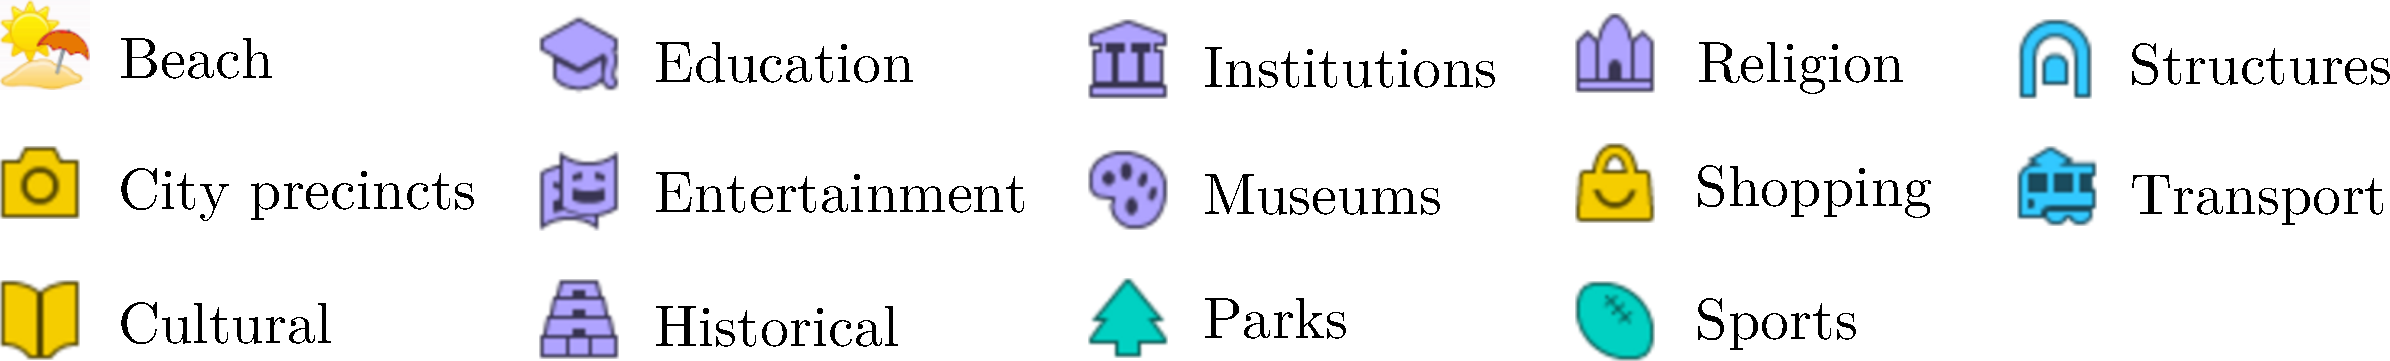
\includegraphics[width=0.7\textwidth]{fig/poi_cats_fat.pdf}
	\caption{POI Categories}
	\label{fig:poicats}
\end{figure*}


\begin{figure*}[t]
\includegraphics[width=\textwidth]{fig/feature_distro.pdf}
\caption{Distribution of POI popularity, the number of visit and visit duration}
\label{fig:distro}\captionmoveup
\end{figure*}



We described an algorithm to recommend trajectories based on ranking POIs (\textsc{PoiRank}) in Section~\ref{sec:rankplan},
the features used to rank POIs are POI and query specific, as described in Table~\ref{tab:featurerank}.

Categories of POIs in all of the five trajectory datasets are show in Figure~\ref{fig:poicats}.
The distribution of POI popularity, the number of visit and average visit duration are shown in Figure~\ref{fig:distro}.

To rank POIs, features described in Table~\ref{tab:featurerank} are scaled to range $[-1.0, 1.0]$ using the same approach 
as that utilised by libsvm (\url{http://www.csie.ntu.edu.tw/~cjlin/libsvm/}),
i.e., fitting a linear function $f(x) = a x + b$ for feature $x$ such that the maximum value of $x$ maps to $1.0$ 
and the minimum value of $x$ maps to $-1.0$.



\section{Transition Probabilities}

\begin{table}[ht]
\caption{POI features used to factorise POI-POI transition probabilities}
\label{tab:featuretran}
\centering
\setlength{\tabcolsep}{28pt} % tweak the space between columns
\begin{tabular}{l|l} \hline
\textbf{Feature}       & \textbf{Description} \\ \hline
\texttt{category}      & category of POI \\
\texttt{neighbourhood} & the cluster that a POI resides in \\
\texttt{popularity}    & (discretised) popularity of POI \\
\texttt{nVisit}        & (discretised) total number of visit at POI \\
\texttt{avgDuration}   & (discretised) average duration at POI \\ \hline
\end{tabular}
\end{table}


\begin{figure*}[b]
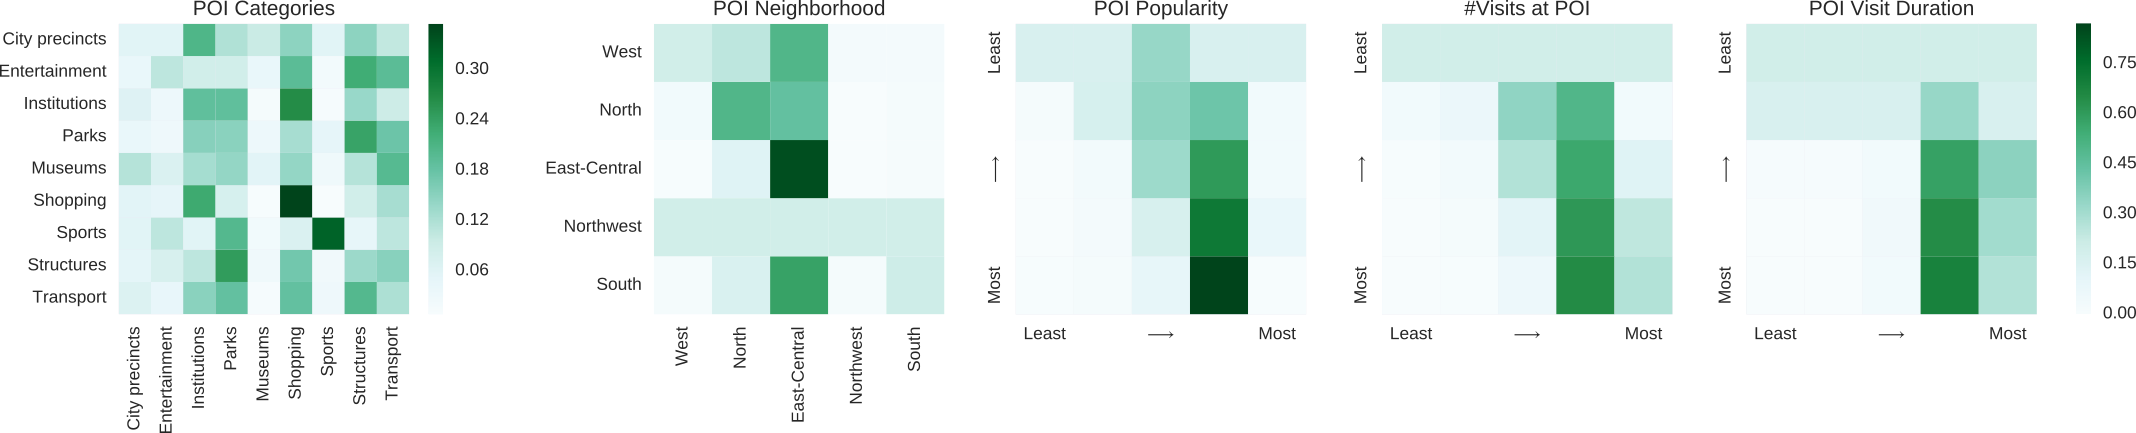
\includegraphics[width=\textwidth]{fig/poi_transmat_all.png}
\caption{Transition matrices for five POI features: POI categories, neighborhood, popularity, number of visits, and visit duration. These statistics are from the Melbourne dataset.}
\label{fig:transmat_all}
\end{figure*}

We compute the POI-POI transition matrix by factorising transition probabilities from POI $p_i$ to POI $p_j$ as a product of transition probabilities
between pairs of individual POI features, these features are described in Table~\ref{tab:featuretran}.

Transition matrices of individual POI features are computed using maximum likelihood estimation,
i.e., counting the number of transitions for each pair of features then normalising each row,
taking care of zeros by adding a small number $\epsilon$
\footnote{In our experiments, $\epsilon = 1$.}
to each count before normalisation.
Figure~\ref{fig:transmat_all} visualises the transition matrices for individual POI features in Melbourne.

The POI-POI transition matrix is computed by taking the Kronecker product of the transition matrices for the individual features,
and then updating it with two additional constraints.

Firstly, we disallow self transitions by setting probability of ($p_i$ to $p_i$) to zero.

Secondly, when a group of POIs have identical (discretised) features (say a group with $N_g$ POIs), 
we distribute the probability uniformly among POIs in the group,
in particular, the incoming (unnormalised) transition probability (say, $P_i$) of the group computed by taking the Kronecker product is divided uniformly 
among POIs in the group (i.e., $\frac{P_i}{N_g}$), which is equivalent to choose a POI in the group uniformly at random.
Moreover, the outgoing (unnormalised) transition probability of each POI is the same as that of the group, 
since in this case, \textit{the transition from any POI in the group to one outside the group represents an outgoing transition from that group}.
In addition, the self-loop transition of the group represents transitions from a POI in the group to other POIs ($N_g-1$ POIs) in the same group, 
\textit{similar to the outgoing case}, the (unnormalised) self-loop transition probability (say $P_o$) is divided uniformly (i.e., $\frac{P_o}{N_g-1}$),
which corresponds to choose a transition (from $p_i$) among all transitions to the other $N_g-1$ POIs (exclude self-loop $p_i$ to $p_i$)
in that group uniformly at random.

Lastly, we normalise each row of the (unnormalised) POI-POI transition matrix to form a valid probability distribution for each POI.



\section{Experiment}

\subsection{Dataset}
Trajectories used in experiment are extracted using geo-tagged photos in the Yahoo! Flickr Creative Commons 100M
(a.k.a. YFCC100M) dataset~\cite{thomee2016yfcc100m} as well as the Wikipedia web-pages of points-of-interests (POIs).
Photos are mapped to POIs according to their distances calculated using the Haversine formula~\cite{haversine},
the time a user arrived a POI is approximated by the time the first photo taken by the user at that POI,
similarly, the time a user left a POI is approximated by the time the last photo taken
by the user at that POI.
Furthermore, sequence of POI visits by a specific user are divided into several pieces according to
the time gap between consecutive POI visits, and the POI visits in each piece are connected in temporal order
to form a trajectory~\cite{ht10, ijcai15}.

\subsection{Parameters}
For parameters of algorithms in experiment,
we use a $0.5$ trade-off parameter for \textsc{PersTour} and \textsc{PersTour-L}, found to be the best weighting by \textsc{PersTour}~\cite{ijcai15}.
The regularisation parameter $C$ in rankSVM is $10.0$.
The trade-off parameter $\alpha$ in \textsc{Rank+Markov} and \textsc{Rank+MarkovPath} is tuned using cross validation.
In particular, we split trajectories with more than $2$ POIs in a dataset into two (roughly) equal parts, 
and use the first part (i.e., validation set) to tune $\alpha$ (i.e., searching value of $\alpha$ such that \textsc{Rank+Markov} achieves the best performance on validation set, in terms of the mean of pairs-F$_1$ scores got by leave-one-out cross validation),
then test on the second part (leave-one-out cross validation) using the tuned $\alpha$, and vice verse. 

\subsection{Implementation}
We employ the rankSVM implementation in libsvmtools (\url{https://www.csie.ntu.edu.tw/~cjlin/libsvmtools/}).
Integer linear programming (ILP) are solved using Gurobi Optimizer (\url{http://www.gurobi.com/})
and lp\_solve (\url{http://lpsolve.sourceforge.net/}).
Dataset and code for this work are available in repository \url{https://bitbucket.org/d-chen/tour-cikm16}.

\subsection{Performance metric}
A commonly used metric for POI recommendation and evaluating trajectories is
the F$_1$ score on points.
Let $\mathcal{T}$ be the trajectory that was visited in the real world,
and $\hat{\cal T}$ be the recommended trajectory,
$\mathcal{P}_{\mathcal{T}}$ be the set of POIs visited in $\mathcal{T}$,
and $\mathcal{P}_{\hat{\mathcal{T}}}$ be the set of POIs visited in $\hat{\mathcal{T}}$,
we compute F$_1$ score on points as the harmonic mean between the point-wise precision and recall,
%was defined as
\begin{displaymath}
F_1= \frac{2  P_{\textsc{point}}  R_{\textsc{point}}}
          {P_{\textsc{point}} + R_{\textsc{point}}}
\end{displaymath}
where
\vspace{-1.1em}
\begin{displaymath}%\eqmoveup
P_{\textsc{point}} = \frac{|\mathcal{P}_{\mathcal{T}} \cap \mathcal{P}_{\hat{\mathcal{T}}}|}
                          {|\hat{\mathcal{T}}|},
R_{\textsc{point}} = \frac{|\mathcal{P}_{\mathcal{T}} \cap \mathcal{P}_{\hat{\mathcal{T}}}|}
                          {|\mathcal{T}|}
\end{displaymath}

A perfect F$_1$ (i.e., F$_1 = 1$) means the POIs in
the recommended trajectory are exactly the same POIs as those in the ground truth,
and F$_1 = 0$ means that none of the POIs in the
real trajectory was recommended.

While F$_1$ score on points is good at measuring whether POIs are correctly recommended,
it ignores the visiting order between POIs.
$\text{pairs-F}_1$ takes into account both the point identity and the visiting orders in a trajectory.
This is done by measuring the F$_1$ score of every pair of ordered POIs, whether they are adjacent or not,
\begin{displaymath}
\text{pairs-F}_1 = \frac{2 P_{\textsc{pair}} R_{\textsc{pair}}}
                        {P_{\textsc{pair}} + R_{\textsc{pair}}},
\end{displaymath}
where
\vspace{-2.0em}
\begin{displaymath}%\eqmoveup
~~
P_{\textsc{pair}} = \frac{N_c} {|\hat{\mathcal{T}}|(|\hat{\mathcal{T}}|-1) / 2}, ~~
R_{\textsc{pair}} = \frac{N_c} {|\mathcal{T}|(|\mathcal{T}|-1) / 2},
\end{displaymath}
and $N_c$
\footnote{We define pairs-F$_1 = 0$ when $N_c = 0$.}
is the number of ordered POI pairs $(p_j, p_k)$ that
appear in both the ground-truth and the recommended trajectories,
\begin{align*}
    (p_j \prec_{\mathcal{T}} p_k ~\land~ p_j \prec_{\hat{\mathcal{T}}} p_k)  ~\lor~
    (p_j \succ_{\mathcal{T}} p_k ~\land~ p_j \succ_{\hat{\mathcal{T}}} p_k),
\end{align*}
with $p_j \ne p_k, ~p_j, p_k \in \mathcal{P}_{\mathcal{T}} \cap \mathcal{P}_{\hat{\mathcal{T}}}, ~1 \le j \ne k \le |\mathcal{T}|$.
Here $p_j \prec_{\mathcal{T}} p_k$ denotes POI $p_j$ was visited before POI $p_k$ in trajectory $\mathcal{T}$
and $p_j \succ_{\mathcal{T}} p_k$ denotes $p_j$ was visited after $p_k$ in $\mathcal{T}$.

Pairs-F$_1$ takes values between 0 and 1. A perfect pairs-F$_1$ (1.0) is achieved if and only if
both the POIs and their visiting orders in the recommended trajectory are exactly the same as those in the ground truth.
Pairs-F$_1 = 0$ means none of the recommended POI pairs was actually visited in the real trajectory.

Performance data reported in Table~\ref{tab:f1} and Table~\ref{tab:pairf1} are the mean and standard deviation of instances successfully recommended by
all methods shown in Table~\ref{tab:algsummary}.




\eat{
%\cheng{Report the proportion of recommended trajectories and actual trajectories with sub-tours, in the Appendix.}


\section{Markov}

\begin{algorithm}[t]
\caption{\textsc{Markov}: recommend trajectory with POI transitions}
%recommend trajectory by maximising likelihood}
\label{alg:markov}
\begin{algorithmic}[1]
\STATE \textbf{Input}: $\mathcal{P}, p_s, p_e, L$
\STATE \textbf{Output}: Trajectory $\mathcal{T} = (p_s, \cdots, p_e)$ with $L$ POIs
%\STATE Compute POI-POI transition matrix
\STATE Initialise score matrix $A$ and backtracking pointer $B$
\FOR{$p \in \mathcal{P}$}
    \STATE $A[2, p] = \log P(p|p_s)$
    \STATE $B[2, p] = p_s$
\ENDFOR
\FOR{$l=2$ to $L-1$}
    \FOR{$p \in \mathcal{P}$}
        \STATE \(\displaystyle A[l+1, p] = \max_{p' \in \mathcal{P}} \{ A[l, p'] + \log P(p|p') \} \)
        \STATE \(\displaystyle B[l+1, p] = \argmax_{p' \in \mathcal{P}} \{ A[l, p'] + \log P(p|p') \} \)
    \ENDFOR
\ENDFOR
% //trace back to find the actual path
\STATE $\mathcal{T} = \{p_e\}$, $l = L$, $p = \mathcal{T}.first$
\REPEAT
    \STATE Prepend $B[l, p]$ to $\mathcal{T}$
    \STATE $l = l - 1$, $p = \mathcal{T}.first$
\UNTIL{$l < 2$}
\RETURN $\mathcal{T}$
\end{algorithmic}
\end{algorithm}





\section{Avoid Peeking}
When working with machine learning algorithms, to make sure the reported performance is a good approximation
of the generalisation performance, it is critical to prevent information in test set from leaking into
training set.
Many algorithms shown in Table~\ref{tab:algsummary} leveraging both learning to rank and 
factorised POI-POI transition matrix,
e.g., \textsc{Rank+Markov}, \textsc{Rank+MarkovPath} and \textsc{StructuredSVM},
both of them need to be trained or parameters be estimated before being utilised in other algorithms.
POI features such as popularity, the number of visits and average visit duration are
determined by not only the POI itself but also trajectories in training set, 
let's call them aggregated features, as they are computed by aggregating a set of trajectories.
To make sure the prediction performance is reliable, 
it is very important to exclude trajectories in test set when computing aggregated features.
Unfortunately, it is quite easy, especially when utilising multiple levels of machine learning models,
to use all data, including those in test set, to compute aggregated features, 
and many researchers and practitioners did not realise the fact that 
some bits of information in test set were leaked into training set via these aggregated features.

%One may argue that many of these features will not change much when computed with or without data in test set,
%but in certain areas, such as aerodynamics, some decisions are very sensitive to the quantity of certain features.
%Nevertheless, the exact impact still needs further investigation.





\section{RankSVM}
\label{appendix:ranksvm}

\subsection{Prediction}
Given a set of $M$ POIs $\mathcal{P} = \{p_1, \cdots, p_M\}$, 
and $N$ queries $\mathcal{Q} = \{q_1, \cdots, q_N\}$.
The ranking score for POI $p_m$ with respect to query $q_n$ is 
$S_{m,n} = \langle \mathbf{w_r}, \mathbf{\phi}(p_m, q_n) \rangle$,
where $\mathbf{w_r}$ is a vector of parameters,
and $\mathbf{\phi}(p_m, q_n)$ is the scaled feature vector for $p_m$ with respect to query $q_n$,
as described in Table~\ref{tab:featurerank}.

\subsection{Training}
To estimate the parameters $\mathbf{w_r}$, we train a rankSVM with linear kernel and L$2$ loss:
%\begin{displaymath}
\begin{multline}
\min_{\mathbf{w_r}} \frac{1}{2} \mathbf{w_r}^T \mathbf{w_r} + \\ \hfill
                    C_r \sum_{(p_i, q_n), (p_j, q_n) \in \mathcal{P} \times \mathcal{Q}}
                    \max \left( 0, 1 - \mathbf{w_r}^T (\mathbf{\phi}(p_i, q_n) - \mathbf{\phi}(p_j, q_n)) \right)^2
\end{multline}
%\end{displaymath}
where $C_r > 0$ is the regularisation parameter.

The label of a training example is the number of occurrences of POI $p_m$ in trajectories grouped by query $q = (p_s, p_e, L)$,
without counting the occurrence of $p_m$ when it is the origin or destination of a trajectory.


\subsection{Structured SVM}
\label{sec:ssvm}
\secmoveup

As trajectory is a sequence of POI visits,
it is natural to model the recommended trajectory $\mathcal{T}$ with respect to query $q = (p_s, p_e, L)$
as a chain of $L$ variables, where each discrete variable has $|\mathcal{P}|$ states.
Structured prediction incorporates both the features of variables (unary features) and
the features of interactions between neighbouring variables (pairwise features) to make a
prediction,
\begin{displaymath}
    \mathcal{T}^* = \argmax_{\mathcal{T} \in \mathcal{P}^L} 
                    \sum_{j=1}^L \mathbf{w_u}^T \mathbf{\phi}_j \left( q, \mathcal{T}_j \right) +
                    \sum_{j=1}^{L-1} \mathbf{w_p}^T \mathbf{\phi}_{j, j+1} \left( q, \mathcal{T}_j, \mathcal{T}_{j+1} \right)
\end{displaymath}
where $\mathbf{\phi}_j$ are the unary features of the $j$-th variable and $\mathbf{\phi}_{j, j+1}$ are the pairwise features between
the $j$-th and $(j+1)$-th variables, $\mathbf{w_u}$ and $\mathbf{w_p}$ are the
parameters of unary and pairwise features respectively.

The unary and pairwise features are constructed from the POI ranking and POI-POI transitions.
In particular, unary features are defined as ranking probabilities (Equation~\ref{eq:poi-probability}).
Recall that we have a query consisting of start ($p_s$) and end ($p_e$) locations, which
we model as a 1-of-$K$ encoding in the unary features.
The pairwise features are defined from the transition probabilities $P(p_j | p_i)$ described in
Section~\ref{sec:transition}.
This method is called \textsc{StructuredSVM} in the experiments.

% describe SSVM training (1-slack formulation)
To estimate the parameters $\mathbf{w_u}$ and $\mathbf{w_p}$, we train a Structured Support Vector Machine
using the 1-slack formulation~\cite{ssvm09},
\begin{align*}
    \min_{\mathbf{w}, \xi \ge 0} ~~& \frac{1}{2} \mathbf{w}^T \mathbf{w} + C \xi \\
    s.t. ~~& \forall \left( \hat{\mathcal{T}}^{(1)}, \cdots, \hat{\mathcal{T}}^{(N)} \right) \in \mathscr{T}^N: \\
         ~~& \frac{1}{N} \mathbf{w}^T \sum_{i=1}^N \delta \left( \hat{\mathcal{T}}^{(i)} \right) \ge
             \frac{1}{N} \sum_{i=1}^N \Delta \left( \mathcal{T}^{(i)}, \hat{\mathcal{T}}^{(i)} \right) - \xi \\
%         ~~& \forall \hat{\mathcal{T}}^{(i)} \in \mathcal{P}^{|\mathcal{T}^{(i)}|}, i = 1, \cdots, N
\end{align*}
where $\mathbf{w} = [\mathbf{w_u}^T, \mathbf{w_p}^T]^T$ is the parameter vector,
$\mathcal{T}^{(i)}$ and $\hat{\mathcal{T}}^{(i)}$ are the $i$-th trajectory in training set
and its corresponding recommendation respectively.
$N$ is the training set size, $C$ is the regularisation parameter,
$\xi$ is the slack variable, and
\begin{displaymath}
    \delta \left( \hat{\mathcal{T}}^{(i)} \right) = \Psi \left( q^{(i)}, \mathcal{T}^{(i)} \right) - 
                                                    \Psi \left( q^{(i)}, \hat{\mathcal{T}}^{(i)} \right)
\end{displaymath}
where $q^{(i)}$ the query corresponds to the $i$-th trajectory in training set,
$\Psi \left( q^{(i)}, \mathcal{T}^{(i)} \right)$ is the joint feature vector which is a composite of unary and 
pairwise features of the $i$-th trajectory,
$\Delta \left( \mathcal{T}^{(i)}, \hat{\mathcal{T}}^{(i)} \right)$ is the loss associated with the $i$-th trajectory 
and its corresponding recommendation, and Hamming loss is used in this work.



\section{Structured SVM}
\label{appendix:ssvm}

To recommend a trajectory that starts from POI $p_s$, ends at POI $p_e$, and with $L$ POIs in total.
We build a chain with $L$ random variables (nodes) and $L-1$ directed edges between neighbouring variables,
each discrete variable has $|\mathcal{P}|$ states.
Both the first variable and the last variable are observed, i.e., they are $p_s$ and $p_e$ respectively,
all intermediate variables corresponds to POIs that should be recommended.


\subsection{Node Features}
\label{appendix:node}
Given a POI $p_m$ and a query $q_n$, the node features are the same as that described in Table~\ref{tab:featurerank}.
Features are scaled the same way as that described in Section~\ref{appendix:ranksvm}.


\subsection{Edge Features}
\label{appendix:edge}
Given an ordered pair of POIs $(p_i, p_j)$, 
the edge/pairwise features are built from the factorised transition probabilities 
according to features described in Table~\ref{tab:featuretran}:
\begin{enumerate}
\item The transition probability from the category of $p_i$ to the category of $p_j$.
\item The transition probability from the cluster with $p_i$ to the cluster with $p_j$.
\item The transition probability from the interval with the popularity of $p_i$ to the interval 
      with the popularity of $p_j$.
\item The transition probability from the interval with the number of visit at $p_i$ to the interval 
      with the number of visit at $p_j$.
\item The transition probability from the interval with the average duration at $p_i$ to the interval 
      with the average duration at $p_j$.
\end{enumerate}


\subsection{Prediction}
Given parameters for node and edge features $\mathbf{w_u}$ and $\mathbf{w_p}$, 
we can compute the score of $\mathcal{T}$ as follows:
\begin{displaymath}
S'(\mathcal{T}) = \sum_{j=1}^L     \langle \mathbf{w_u}, \mathbf{\phi}_j (\mathcal{T}_j, q) \rangle +
                  \sum_{j=1}^{L-1} \langle \mathbf{w_p}, \mathbf{\phi}_{j, j+1} (\mathcal{T}_j, \mathcal{T}_{j+1}) \rangle
\end{displaymath}
where $L = |\mathcal{T}|$ is the length of $\mathcal{T}$, 
$\mathbf{\phi}_j$ is the feature vector of the $j$-th node (variable) described in Section~\ref{appendix:node},
$q$ is the query corresponding to $\mathcal{T}$, i.e., $q = (\mathcal{T}_0, \mathcal{T}_L, L)$,
and $\mathbf{\phi}_{j, j+1}$ is the feature vector of the $j$-th edge, as described in Section~\ref{appendix:edge}.

One approach to recommend a trajectory with respect to query $q = (p_s, p_e, L)$ and parameters 
$\mathbf{w_u}$ and $\mathbf{w_p}$ is recommending the one with the maximum score, i.e.,
\begin{displaymath}
    \mathcal{T}^* = \argmax_{\mathcal{T} \in \mathcal{P}^L} S'(\mathcal{T})
\end{displaymath}


\subsection{Training}
To estimate the parameters $\mathbf{w_u}$ and $\mathbf{w_p}$, we train a Structured Support Vector Machine
using the 1-slack formulation,
\begin{align*}
    \min_{\mathbf{w}, \xi \ge 0} ~~& \frac{1}{2} \mathbf{w}^T \mathbf{w} + C \xi \\
    s.t. ~~& \forall \left( \bar{\mathcal{T}}^{(1)}, \cdots, \bar{\mathcal{T}}^{(N)} \right) \in \mathscr{T}^N: \\
         ~~& \frac{1}{N} \mathbf{w}^T \sum_{i=1}^N \delta \left( \bar{\mathcal{T}}^{(i)} \right) \ge
             \frac{1}{N} \sum_{i=1}^N \Delta \left( \mathcal{T}^{(i)}, \bar{\mathcal{T}}^{(i)} \right) - \xi
\end{align*}
where $\mathbf{w} = [\mathbf{w_u}^T, \mathbf{w_p}^T]^T$ is the parameter vector,
$C > 0$ is the regularisation parameter, $\xi$ is the slack variable, 
$N$ is the number of trajectories in training set, 
$\mathcal{T}^{(i)}$ is the $i$-th trajectory in training set, 
and its corresponding recommendation is $\bar{\mathcal{T}}^{(i)}$, and
\begin{displaymath}
    \delta \left( \bar{\mathcal{T}}^{(i)} \right) = \Psi \left( \mathcal{T}^{(i)}, q^{(i)} \right) - 
                                                    \Psi \left( \bar{\mathcal{T}}^{(i)}, q^{(i)} \right)
\end{displaymath}
where $q^{(i)}$ is the query corresponding to $\mathcal{T}^{(i)}$ and the joint feature vector of $\mathcal{T}^{(i)}$ is
\begin{displaymath}
\Psi \left( \mathcal{T}^{(i)}, q^{(i)} \right) = \left[
\left( \sum_{j=1}^{|\mathcal{T}^{(i)}|}   \mathbf{\phi}_{j}      \left( \mathcal{T}_{j}^{(i)}, q^{(i)} \right) \right)^T,
\left( \sum_{j=1}^{|\mathcal{T}^{(i)}|-1} \mathbf{\phi}_{j, j+1} \left( \mathcal{T}_{j}^{(i)}, \mathcal{T}_{j+1}^{(i)} \right) \right)^T 
\right]^T
\end{displaymath}
$\Delta \left( \mathcal{T}^{(i)}, \bar{\mathcal{T}}^{(i)} \right)$ is the loss associated with the $i$-th trajectory 
and its corresponding recommendation, and Hamming loss is used in our experiment.
}
